\section{Results}
\subsection{Deep Neural Net}
We will now proceed with presenting results for a deep neural net using the Gradient Descent optimizer in table \ref{tab:dnn_general_results_gd}, put together using different hyper parameters. Similar hyper parameters but with the Adam optimizer can be viewed in the table \ref{tab:dnn_general_results_adam}. Combinations where put together from different amount of layers, neurons on each layer, activation functions and optimizers. The results were retrieved running $N_\mathrm{e}=10^5$ epochs. To evaluate the performance we look at the $R^2$ score\eqref{eq:r2} and the MSE score\eqref{eq:mse}. The $\varepsilon_{\mathrm{abs}}=|u - \hat{u}|$, where $u$ is the numerical results and $\hat{u}$ is the analytical results.
\begin{table}[h!tb]
    \centering
    \caption{Results for a DNN with different hyper parameters. The number of epoch was set to $N_\mathrm{e}=10^5$. Results presented are obtained with \textit{gradient descent} as optimizer.}
    \pgfplotstabletypeset[
        every head row/.style={before row=\toprule,after row=\midrule},
        every last row/.style={after row=\bottomrule},
        % columns/optimizer/.style={string type, column name={Optimizer}},
        columns/activation/.style={string type, column name={Activation}},
        columns/layers/.style={column name={Layers}},
        columns/neurons/.style={column name={Neurons}},
        columns/diff/.style={sci, column name=$\mathrm{max}(\varepsilon_{\mathrm{abs}})$},
        columns/r2/.style={sci, column name=$R^2$},
        columns/mse/.style={sci, column name=$MSE$},
        % columns/time/.style={sci, column name=$\Delta t$}
    ]{../results/dnn_general_table_gd.dat}
    \label{tab:dnn_general_results_gd}
\end{table}

\begin{table}[h!tb]
    \centering
    \caption{Results for a DNN with different hyper parameters. The number of epoch was set to $N_\mathrm{e}=10^5$. Results presented are obtained with the \textit{Adam} optimizer\cite{kingma_adam:_2014}.}
    \pgfplotstabletypeset[
        every head row/.style={before row=\toprule,after row=\midrule},
        every last row/.style={after row=\bottomrule},
        % columns/optimizer/.style={string type, column name={Optimizer}},
        columns/activation/.style={string type, column name={Activation}},
        columns/layers/.style={column name={Layers}},
        columns/neurons/.style={column name={Neurons}},
        columns/diff/.style={sci, column name=$\mathrm{max}(\varepsilon_{\mathrm{abs}})$},
        columns/r2/.style={sci, column name=$R^2$},
        columns/mse/.style={sci, column name=$MSE$},
        % columns/time/.style={sci, column name=$\Delta t$}
    ]{../results/dnn_general_table_adam.dat}
    \label{tab:dnn_general_results_adam}
\end{table}


% We also run with a dropout rates of $\epsilon_\mathrm{Dropout}=0.25, 0.5$. The results can be viewed in following table
% \begin{table}[h!tb]
%     \centering
%     \caption{Results for a DNN with different hyper parameters. The number of epoch was set to $N_\mathrm{epochs}=10^5$, and we used a dropout rate of $\epsilon_\mathrm{Dropout}=0.25, 0.5$.}
%     \pgfplotstabletypeset[
%         every head row/.style={before row=\toprule,after row=\midrule},
%         every last row/.style={after row=\bottomrule},
%         columns/optimizer/.style={string type, column name={Optimizer}},
%         columns/activation/.style={string type, column name={Activation}},
%         columns/layers/.style={string type, column name={Layers}},
%         columns/diff/.style={sci, column name=$\mathrm{max}(\varepsilon_{\mathrm{abs}})$},
%         columns/r2/.style={column name=$R^2$},
%         columns/mse/.style={sci, column name=$MSE$},
%         columns/dropout/.style={column name=$\epsilon_\mathrm{Dropout}$}
%     ]{../results/dnn_dropout_table.dat}
%     \label{tab:dnn_dropout_results}
% \end{table}

\subsubsection{Testing out optimal hyper parameters}
From the table \ref{tab:dnn_general_results_adam} with Adam as optimizer, the results which gave us the best $R^2$ and $MSE$ were chosen to be run for $N_\mathrm{e}=10^6$ epochs. The results for this run can be seen in table \ref{tab:dnn_optimal_results_adam}.
\begin{table}[h!tb]
    \centering
    \caption{Results for a DNN $N_\mathrm{e}=10^6$ run with a select set of hyper parameters which yielded the best $R^2$ scores in \ref{tab:dnn_general_results_adam}. Most of the hyper parameters inspected yields a $R^2$ score of more than four repeating digits.}
    \pgfplotstabletypeset[
        every head row/.style={before row=\toprule,after row=\midrule},
        every last row/.style={after row=\bottomrule},
        columns/optimizer/.style={string type, column name={Optimizer}},
        columns/activation/.style={string type, column name={Activation}},
        columns/layers/.style={string type, column name={Layers}},
        columns/diff/.style={sci, column name=$\mathrm{max}(\varepsilon_{\mathrm{abs}})$},
        columns/r2/.style={sci, column name=$R^2$},
        columns/mse/.style={sci, column name=$MSE$},
        columns/duration/.style={sci, column name={Duration}},
    ]{../results/dnn_optimal_table_adam2.dat}
    \label{tab:dnn_optimal_results_adam}
\end{table}

We will use the hyper parameters given in table \ref{tab:dnn_optimal_params} as the optimal settings for our neural network. It is worth mentioning that the exact $R^2$ score this combination provided was $R^2=0.9999999985$. The cost at this point was $\mathcal{C} = 6.74 \cdot 10^{-7}$ based on equation \eqref{eq:pde-cost-function}.
\begin{table}[h!tb]
    \centering
    \caption{Optimal parameters as dictated by table \ref{tab:dnn_optimal_results_adam}.}
    \pgfplotstabletypeset[
        every head row/.style={before row=\toprule,after row=\midrule},
        every last row/.style={after row=\bottomrule},
        columns/optimizer/.style={string type, column name={Optimizer}},
        columns/activation/.style={string type, column name={Activation}},
        columns/layers/.style={string type, column name={Layers}},
        columns/neurons/.style={string type, column name={Neurons}},
    ]{dnn_optimal_params.dat}
    \label{tab:dnn_optimal_params}
\end{table}

\subsubsection{Cost and Error} 
The cost and error of a run with three layers and 10 neurons in each layers run for $10^6$ epochs can be viewed in figure \ref{fig:cost-error}. The error is given as $\max \left( | u_\mathrm{analytic} - u_t | \right)$, where $u_t$ is the numerical approximation by the neural network. The Adam optimizer were used.
\begin{figure}
    \centering
    \includegraphics{../fig/cost_error.pdf}
    \caption{The cost and error as it evolves using hyper parameters given in table \ref{tab:dnn_optimal_params} and $N_\mathrm{e}=10^6$ epochs. Adam was used as an optimizer.}
    \label{fig:cost-error}
\end{figure}

% \subsection{Forward Euler and finite difference}


\subsection{Comparing DNN and Forward-Euler against the analytic solution}
From the table \ref{tab:dnn_optimal_results_adam}, we will use the hyper parameters as given in table \ref{tab:dnn_optimal_params} in further analysis and comparison against the Forward-Euler finite difference method. The Forward-Euler method was run with $N_x=10$ and $N_t=100$, and a $\alpha=\Delta t / \Delta x^2=0.005$ in order to safely maintain the stability condition.

In figure \ref{fig:analytical-solution} we see the analytical solution as given for by \eqref{eq:pde-analytical-solution} for $N_t=10$ and $N_x=10$.
\begin{figure}[h!tb]
    \centering
    \includegraphics[trim={3.5cm 4.0cm 3.5cm 4.5cm},clip,scale=0.8]{../fig/dnn_optimal_3d/analytical_3d_Nt10_Nlayers1_neurons1000_acttanh_optadam_dropout0_0.pdf}
    \caption{The analytical solution as given by \eqref{eq:pde-analytical-solution} for $N_t=10$ and $N_x=10$.}
    \label{fig:analytical-solution}
\end{figure}

In figure \ref{fig:3d-fw-comparison-plots} we see the results from the Forward-Euler method together with the absolute difference between the analytical solution as given by \eqref{eq:pde-analytical-solution}. Comparing with the analytical, we have $R^2=-0.12$ and $MSE=9.87\cdot 10^{-4}$
\begin{figure}[h!tb]
    \centering
    \begin{subfigure}{0.5\textwidth}
        \centering
        \includegraphics[trim={3.5cm 4.0cm 3.5cm 4.5cm},clip,scale=0.45]{../fig/fw_3d/analytical_3d_Nt100.pdf}
        \caption{Forward-Euler.}
        \label{fig:fw-3d}
    \end{subfigure}
    \begin{subfigure}{0.5\textwidth}
        \centering
        \includegraphics[trim={3.5cm 4.0cm 3.5cm 4.5cm},clip,scale=0.45]{../fig/fw_3d/fw_ana_diff_3d_Nt100.pdf}
        \caption{Absolute error between analytical and Forward Euler.}
        \label{fig:fw-ana-diff-3d}
    \end{subfigure}
    \caption{The forward Euler results \ref{fig:fw-3d}, and the absolute error between analytical and Forward Euler\ref{fig:fw-ana-diff-3d}. The Forward Euler was run with $N_x=10$ and $N_t=100$ and $\alpha=\Delta t / \Delta x^2=0.5$.}
    \label{fig:3d-fw-comparison-plots}
\end{figure}

As an example, an increased spatial resolution can be seen in figure \ref{fig:3d-fw-comparison-plots-spatial-highres}. This yielded $R^2=0.88$ and $MSE=1.01\cdot 10^{-5}$.
\begin{figure}[h!tb]
    \centering
    \begin{subfigure}{0.5\textwidth}
        \centering
        \includegraphics[trim={3.5cm 4.0cm 3.5cm 4.5cm},clip,scale=0.45]{../fig/fw_3d/analytical_3d_Nt10000_Nx100.png}
        \caption{Forward-Euler.}
        \label{fig:fw-3d-highres}
    \end{subfigure}
    \begin{subfigure}{0.5\textwidth}
        \centering
        \includegraphics[trim={3.5cm 4.0cm 3.5cm 4.5cm},clip,scale=0.45]{../fig/fw_3d/fw_ana_diff_3d_Nt10000_Nx100.png}
        \caption{Absolute error between analytical and Forward Euler.}
        \label{fig:fw-ana-diff-3d-highres}
    \end{subfigure}
    \caption{The forward Euler results \ref{fig:fw-3d}, and the absolute error between analytical and Forward Euler\ref{fig:fw-ana-diff-3d}. The Forward Euler was run with $N_x=100$ and $N_t=10000$ and $\alpha=\Delta t / \Delta x^2=0.5$.}
    \label{fig:3d-fw-comparison-plots-spatial-highres}
\end{figure}

In figure \ref{fig:3d-dnn-comparison-plots} we see the resulting surface plot given by the neural net for a optimal set of parameters\ref{tab:dnn_optimal_params}.
\begin{figure}[h!tb]
    \centering
    \begin{subfigure}{0.5\textwidth}
        \centering
        \includegraphics[trim={3.5cm 4.0cm 3.5cm 4.5cm},clip,scale=0.45]{../fig/dnn_optimal_3d/dnn_3d_Nt10_Nlayers1_neurons50_acttanh_optadam_dropout0_0.pdf}
        \caption{Neural Network.}
        \label{fig:neural-net-optimal-3d}
    \end{subfigure} \qquad \qquad \qquad
    \begin{subfigure}{0.5\textwidth}
        \centering
        \includegraphics[trim={3.5cm 4.0cm 3.5cm 4.5cm},clip,scale=0.45]{../fig/dnn_optimal_3d/dnn_ana_diff_3d_Nt10_Nlayers1_neurons50_acttanh_optadam_dropout0_0.pdf}
        \caption{Absolute difference between neural network and analytical results.}
        \label{fig:dnn-ana-diff-3d}
    \end{subfigure}
    \caption{The neural net results\ref{fig:neural-net-optimal-3d} and the absolute difference between the neural net and the analytical results\ref{fig:dnn-ana-diff-3d}. Results run for $N_x=10$ and $N_t=10$, with the Adam optimizer, one hidden layer of 50 neurons and $\tanh$ as activation function.}
    \label{fig:3d-dnn-comparison-plots}
\end{figure}


% We can now select a set of time slices, and inspect those further. Figures 

\subsection{Timing}
A quick plot of different timing values for both Forward Euler and the neural net can be viewed in figure \ref{fig:tf-fw-timing-values}. The DNN was run for $10^5$ epochs.
\begin{figure}[h!tb]
    \centering
    \begin{subfigure}{0.5\textwidth}
        \centering
        \includegraphics[scale=0.5]{../fig/timing_tf.pdf}
        \caption{TensorFlow timing values.}
        \label{fig:tf-timing}
    \end{subfigure}
    \begin{subfigure}{0.5\textwidth}
        \centering
        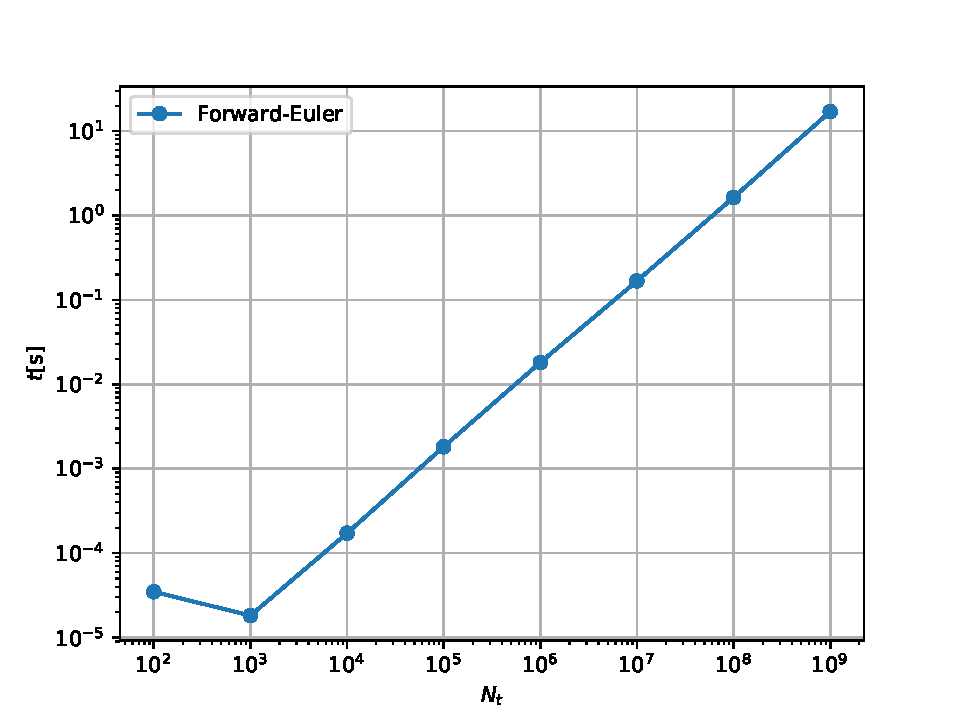
\includegraphics[scale=0.5]{../fig/timing_fw.pdf}
        \caption{Forward Euler timing values.}
        \label{fig:fw-timing}
    \end{subfigure}
    \caption{Timing values for Forward Euler and Neural Net output. The Neural network was calculated using Adam and Sigmoidal activation function. Note, that we are not comparing the same values along the $x$-axis.}
    \label{fig:tf-fw-timing-values}
\end{figure}
